\documentclass[../../main.tex]{subfiles}
\begin{document}

底の断面の形が曲線 $y=x^4-6p^2x^2-8q^3x$ $(p>0,q\geqq0)$ の形の容器がある．
($y$ 軸は鉛直，正の方向を上方にとり，$x$ 軸は水平にとる．)
最初 $q=0$ のときは，大体下図の形になっているので，図の点 $A$ の位置に小球をおく．
ここで，$p$ は固定したまま，$q$ の値をだんだん大きくしていって，ある値を越えたら，この小球は右側のくぼみに転落した．
この値を $p$ を用いて表わせ．

\begin{figure}[htbp]
  \centering
  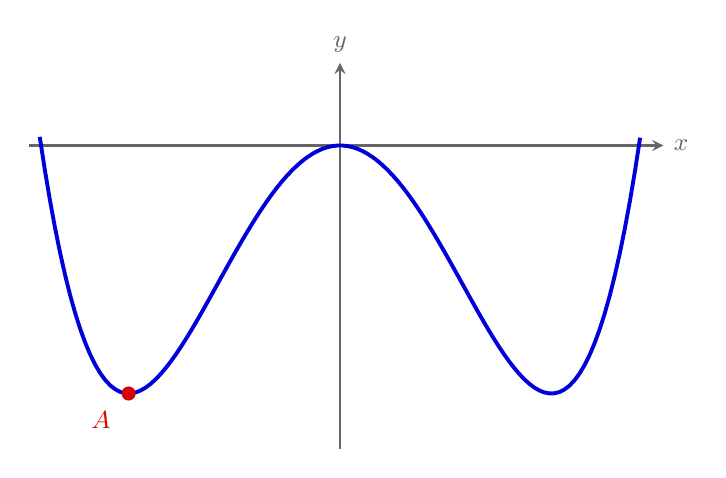
\begin{tikzpicture}[x=1.55cm, y=0.35cm, >=stealth,
    every node/.style={font=\small}]
    % A representative shape for q=0, with p=1.
    \coordinate (A) at ({-sqrt(3)},-9);
    \draw[->, thick, gray!80!black] (-2.55,0) -- (2.65,0) node[right] {$x$};
    \draw[->, thick, gray!80!black] (0,-11) -- (0,3) node[above] {$y$};
    \draw[line width=1.4pt, blue!85!black, domain=-2.46:2.46, samples=120]
    plot (\x,{\x*\x*\x*\x-6*\x*\x});
    \node[circle, fill=red!85!black, inner sep=1.8pt] at (A) {};
    \node[below left=3pt, red!85!black] at (A) {$A$};
  \end{tikzpicture}
  \caption{$q=0$ のときの容器の断面と小球の初期位置 $A$}
\end{figure}

\end{document}
